\documentclass[12pt,a4paper]{article}
\usepackage[utf8]{inputenc}
\usepackage[margin=1in]{geometry}
\usepackage{graphicx}
\usepackage{float}
\usepackage{amsmath}
\usepackage{listings}
\usepackage{xcolor}
\usepackage{enumitem}

% Code listing style
\lstset{
    language=C++,
    basicstyle=\ttfamily\footnotesize,
    keywordstyle=\color{blue},
    commentstyle=\color{green},
    stringstyle=\color{red},
    numbers=left,
    numberstyle=\tiny,
    frame=single,
    breaklines=true
}

\begin{document}

% Front Page
\begin{titlepage}
  \centering
  \vspace*{3cm}

  {\Huge\bfseries CSE 406 – Lab Report 5: Disk Scheduling using FCFS (First Come First Serve) \par}
  \vspace{2.5cm}

  \noindent
  \begin{minipage}[t]{0.48\textwidth}
    {\large\bfseries Submitted By:}\\[0.5em]
    \Large
    Sharif Md. Yousuf \\
    ID: 22101128 \\
    Section: C-2 \\
    4th Year, 1st Semester \\
    Spring 2025
  \end{minipage}
  \hfill
  \begin{minipage}[t]{0.48\textwidth}
    {\large\bfseries Submitted To:}\\[0.5em]
    \Large
    Atia Rahman Orthi \\
    Lecturer \\
    Department of Computer Science \& Engineering \\
    University of Asia Pacific
  \end{minipage}

  \vfill

  {\Large\bfseries Date of Submission:} \\[0.5em]
  {\LARGE\bfseries 16 August, 2025 (Saturday)}

  \vspace*{2cm}
\end{titlepage}

\section{Problem Statement}
In this lab, I was tasked with implementing a disk head scheduling simulator using the First Come First Serve (FCFS) algorithm. The challenge was to create a program that, given an initial head position and a list of pending cylinder requests, would serve these requests in the exact order they arrive - following the first in, first out principle. My program needed to output the order in which requests are served and calculate the total head movement.

\subsection*{Input}
For my implementation, I used:
\begin{itemize}
  \item A predefined sequence of disk cylinder requests
  \item An initial head position
\end{itemize}

Here's what I worked with:
\begin{verbatim}
Request sequence: {11, 34, 41, 50, 52, 69, 70, 114}
Initial head position: 50
\end{verbatim}

\subsection*{Output}
My program produces:
\begin{itemize}
  \item The order in which requests are serviced (FCFS sequence)
  \item Total head movement distance
\end{itemize}

Here's what my program outputs:
\begin{verbatim}
Request Order (FCFS served):
11 34 41 50 52 69 70 114
Total Head Movement: 208
\end{verbatim}

\section{Objective}
Through this lab, I aimed to achieve several learning goals:
\begin{itemize}
    \item Gain a deep understanding of the fundamental disk scheduling algorithm: First Come First Serve (FCFS)
    \item Successfully implement FCFS to serve disk requests in their arrival order
    \item Learn how to calculate total head movement for performance analysis
    \item Compare FCFS characteristics with other scheduling algorithms I've studied
    \item Analyze and appreciate the simplicity and fairness properties that make FCFS special
\end{itemize}

\section{Source Code Screenshot}
\begin{figure}[H]
  \centering
  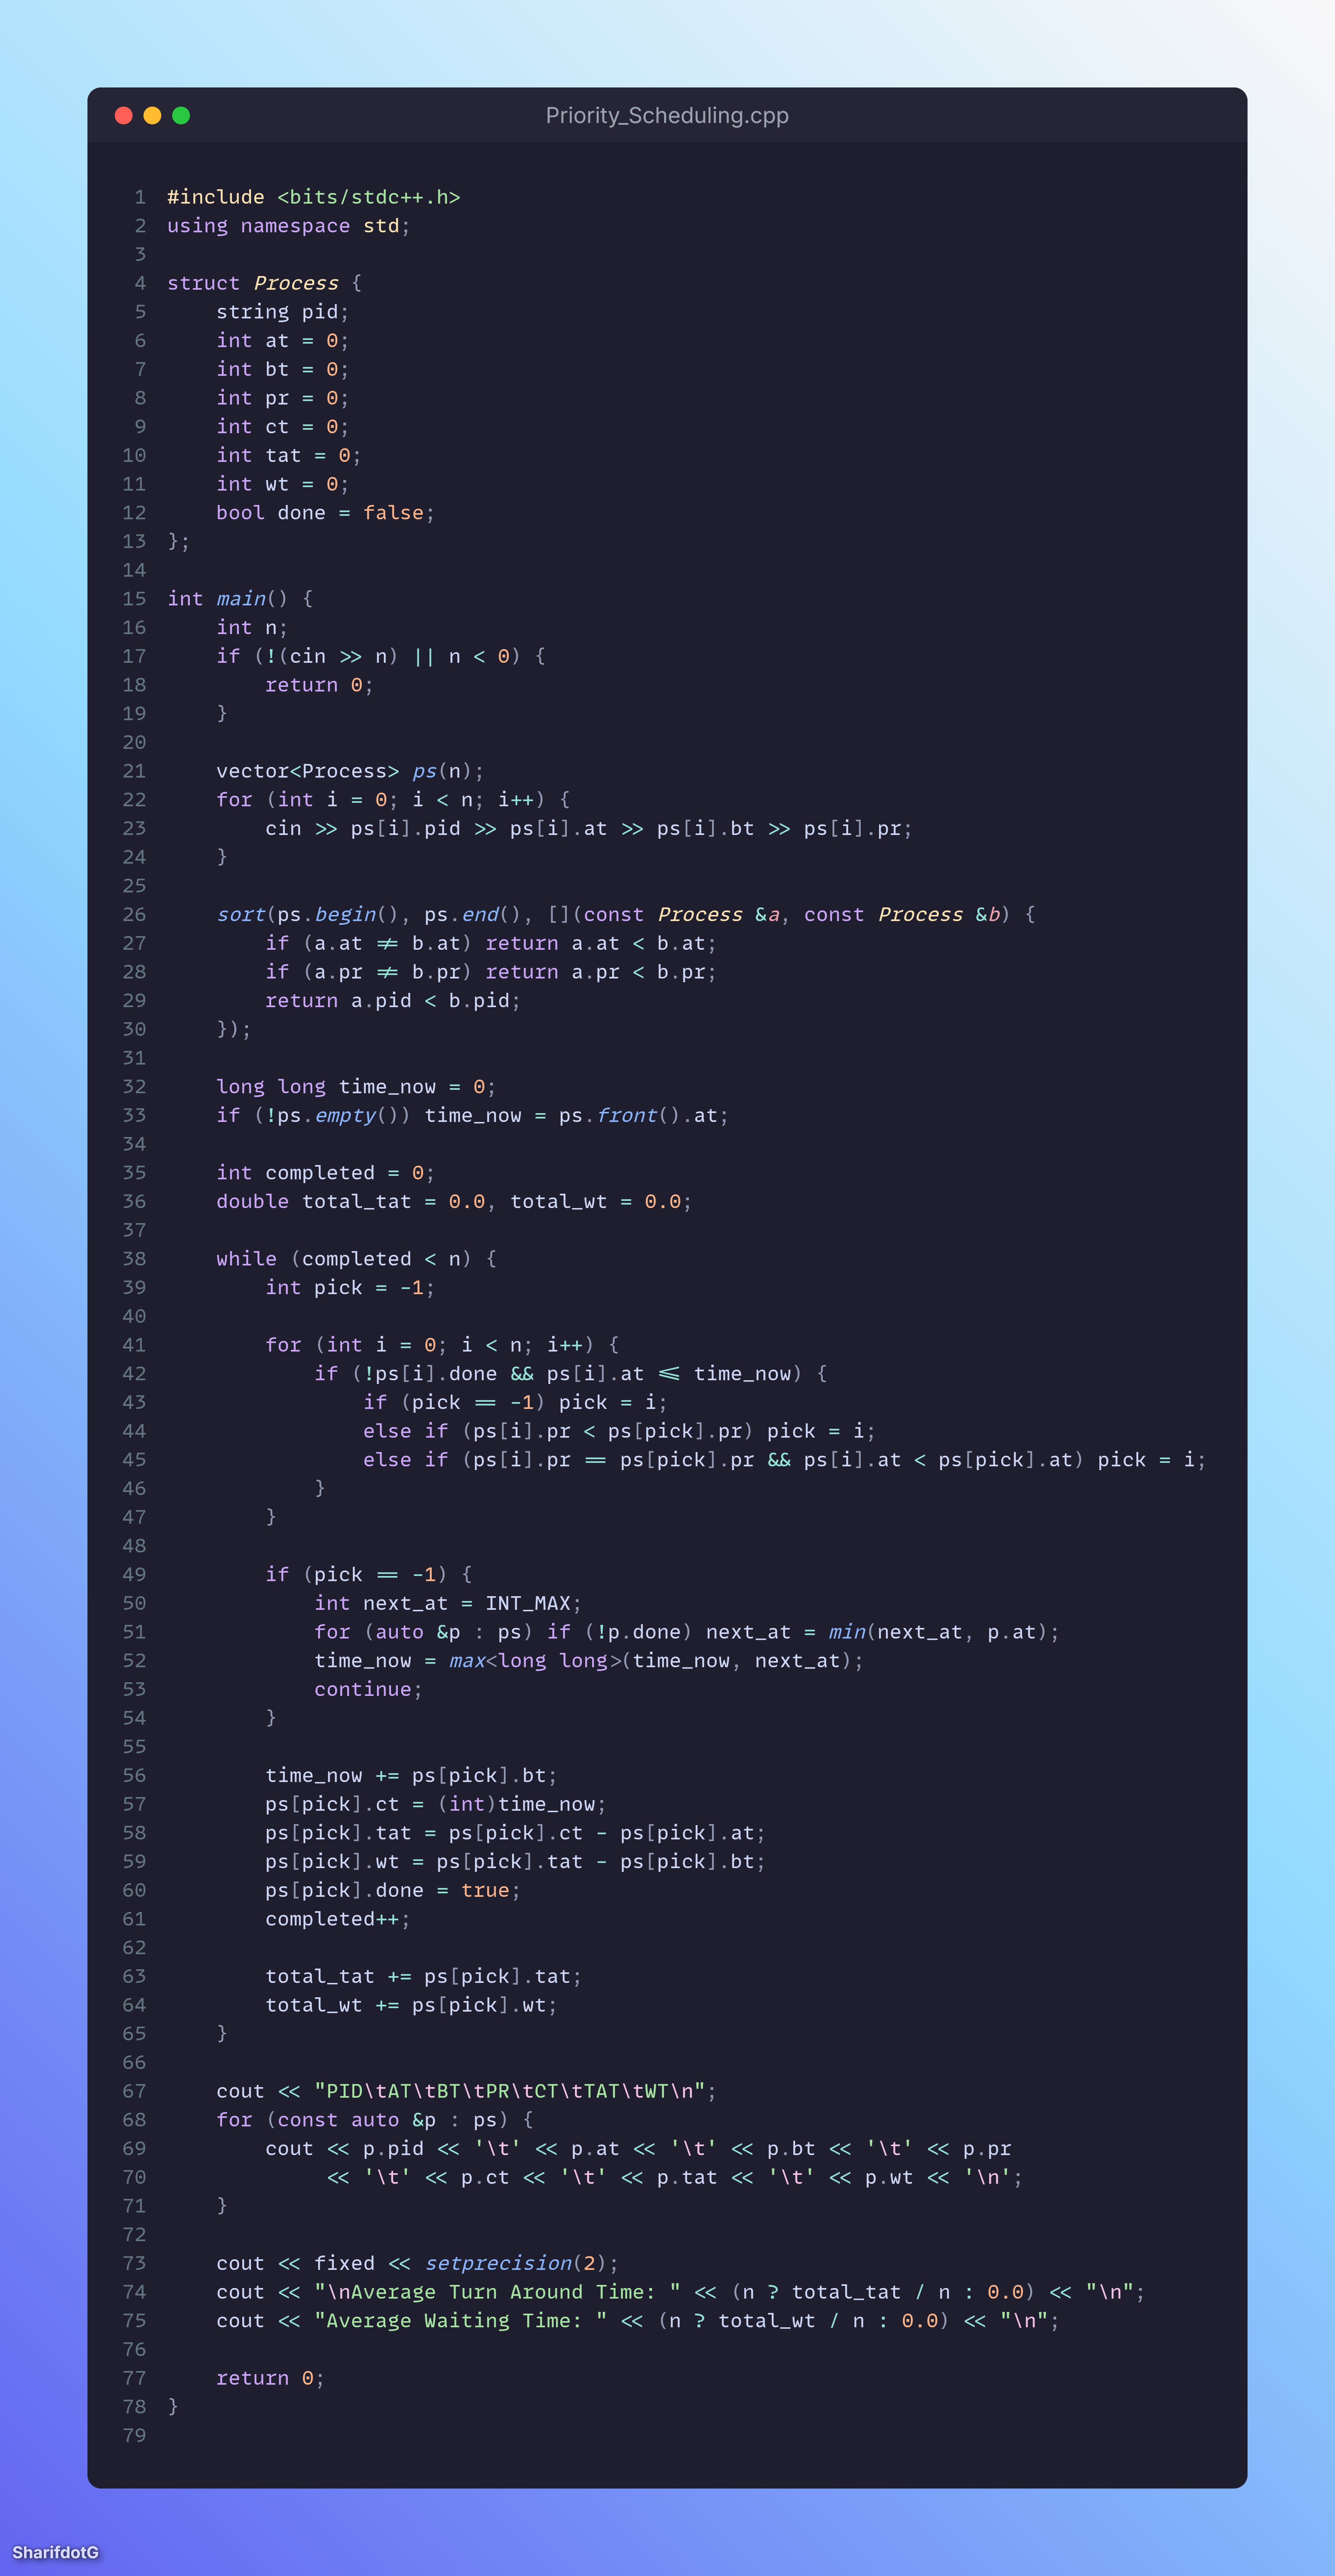
\includegraphics[width=0.85\textwidth]{Code.png}
  \caption{FCFS Disk Scheduling Source Code}
\end{figure}

\section{Output Screenshot}
\begin{figure}[H]
  \centering
  \includegraphics[width=0.85\textwidth]{Screenshot 2025-08-21 163132.png}
  \caption{FCFS Program Output}
\end{figure}

\section{Discussion}
Working with FCFS (First Come First Serve) has been an enlightening experience. I discovered that FCFS is truly the simplest disk scheduling algorithm - it serves requests in the exact order they arrive, without any complex decision-making. Here's what I learned about its key characteristics:

\begin{itemize}
    \item \textbf{Simplicity:} I found it extremely easy to implement and understand. There's no complex decision-making required - just process requests one by one as they come.
    \item \textbf{Fairness:} What I really appreciated is how all requests are treated equally. No request suffers from starvation because each is served in arrival order, which feels very fair.
    \item \textbf{Predictability:} I noticed that response time is completely predictable based on queue position, which makes it reliable from a user perspective.
    \item \textbf{Performance Trade-offs:} However, I observed that this can result in higher total seek time compared to optimized algorithms like SSTF, SCAN, or C-SCAN.
    \item \textbf{No Optimization:} The algorithm doesn't consider the current head position when selecting the next request, which sometimes causes unnecessary long movements.
\end{itemize}

\textbf{My Comparison with Other Algorithms:}
\begin{itemize}
    \item \textbf{vs SSTF:} I realized that FCFS is fairer but typically has higher total seek time. From my studies, I know SSTF can cause starvation for distant requests, which FCFS completely avoids.
    \item \textbf{vs SCAN/C-SCAN:} FCFS is much simpler but less efficient. SCAN algorithms provide better throughput by reducing directional changes, though they're more complex to implement.
    \item \textbf{Real-world Usage:} I learned that FCFS is often used as a baseline for comparison and in scenarios where fairness is more important than performance optimization.
\end{itemize}

Through this implementation, I can see why FCFS serves as an excellent starting point for understanding disk scheduling concepts before exploring more sophisticated algorithms.

\section{Conclusion}
Completing this FCFS disk scheduling implementation has been a valuable learning experience for me. Through this project, I've come to understand the fundamental approach to disk request handling where simplicity and fairness are prioritized over performance optimization.

While I observed that FCFS may not provide the best seek time performance compared to algorithms like SSTF or SCAN, I appreciate how it ensures that no request suffers from starvation and maintains completely predictable behavior. This has given me essential foundational knowledge that I know will help me comprehend more complex disk scheduling algorithms and understand the important trade-offs between performance, fairness, and implementation complexity.

This lab has definitely prepared me well for exploring more advanced scheduling algorithms in the future, and I now have a solid baseline understanding of how disk scheduling works at its most fundamental level.

\end{document}
